%%% PREAMBLE - Do not touch %%%%%%%%%%%%%%%%%%%%%%%%%%%%%%%%%%%%%%%%%%%%%%%%%%%%%%
\documentclass[10pt,twocolumn,letterpaper]{article}
\usepackage[utf8]{inputenc}
\usepackage[english]{babel}
\usepackage{model}
\usepackage{times}
\usepackage{epsfig}
\usepackage{graphicx}
\usepackage{amsmath}
\usepackage{textcomp}
\usepackage{amssymb}
\usepackage{color}
\usepackage[pagebackref=true,breaklinks=true,letterpaper=true,colorlinks,bookmarks=false]{hyperref}

%% inset source code
\usepackage{listings}

\lstset{basicstyle=\footnotesize\ttfamily,  language=C}
\renewcommand{\lstlistingname}{Code}% Listing -> Algorithm

\let\url\nolinkurl% Make \url be equivalent to \nolinkurl
\newcommand*{\Package}[1]{\texttt{#1}}%

\cvprfinalcopy % *** Uncomment this line for the final submission
\def\httilde{\mbox{\tt\raisebox{-.5ex}{\symbol{126}}}}
\ifcvprfinal\pagestyle{empty}\fi

\newcommand{\TODO}[1]{TODO: #1}
\newcommand{\CITEONE}[2]{\mbox{#1 \cite{#2}}}
\newcommand{\CITETWO}[3]{\mbox{#1 and #2 \cite{#3}}}
\newcommand{\CITEN}[2]{\mbox{#1 et al. \cite{#2}}}

%%% Report beginning %%%%%%%%%%%%%%%%%%%%%%%%%%%%%%%%%%%%%%%%%%%%%%%%%%%%%%%%%%%%%%
\begin{document}

%%% Title and authors %%%%%%%%%%%%%%%%%%%%%%%%%%%%%%%%%%%%%%%%%%%%%%%%%%%%%%%%%%%%
\title{Relatório do projeto 1}
\author{Isadora Sophia Garcia Rodopoulos \thanks{RA 158018, Instituto de Computação, Universidade de Campinas, Unicamp. \textbf{Contact}: \tt\small{isadorasophiagr@gmail.com}} \\
Matheus Mortatti Diamantinos \thanks{RA 156740, Instituto de Computação, Universidade de Campinas, Unicamp. \textbf{Contact}: \tt\small{matdiamantino@gmail.com}}\\
Luiz Fernando Bittencourt\thanks{MC833, Instituto de Computação, Universidade de Campinas, Unicamp. \textbf{Contact}: \tt\small{bit@ic.unicamp.br }}\\
}

%%% Abstrato %%%%%%%%%%%%%%%%%%%%%%%%%%%%%%%%%%%%%%%%%%%%%%%%%%%%%%%%%%%%%%%%%%%%%
\maketitle
\begin{abstract}
O objetivo do trabalho se baseou em implementar uma estrutura de cliente e servidor que interagissem entre si.
\end{abstract}

%%% image for demo! %%%%%%%%%% 
\begin{figure*}
\begin{center}
    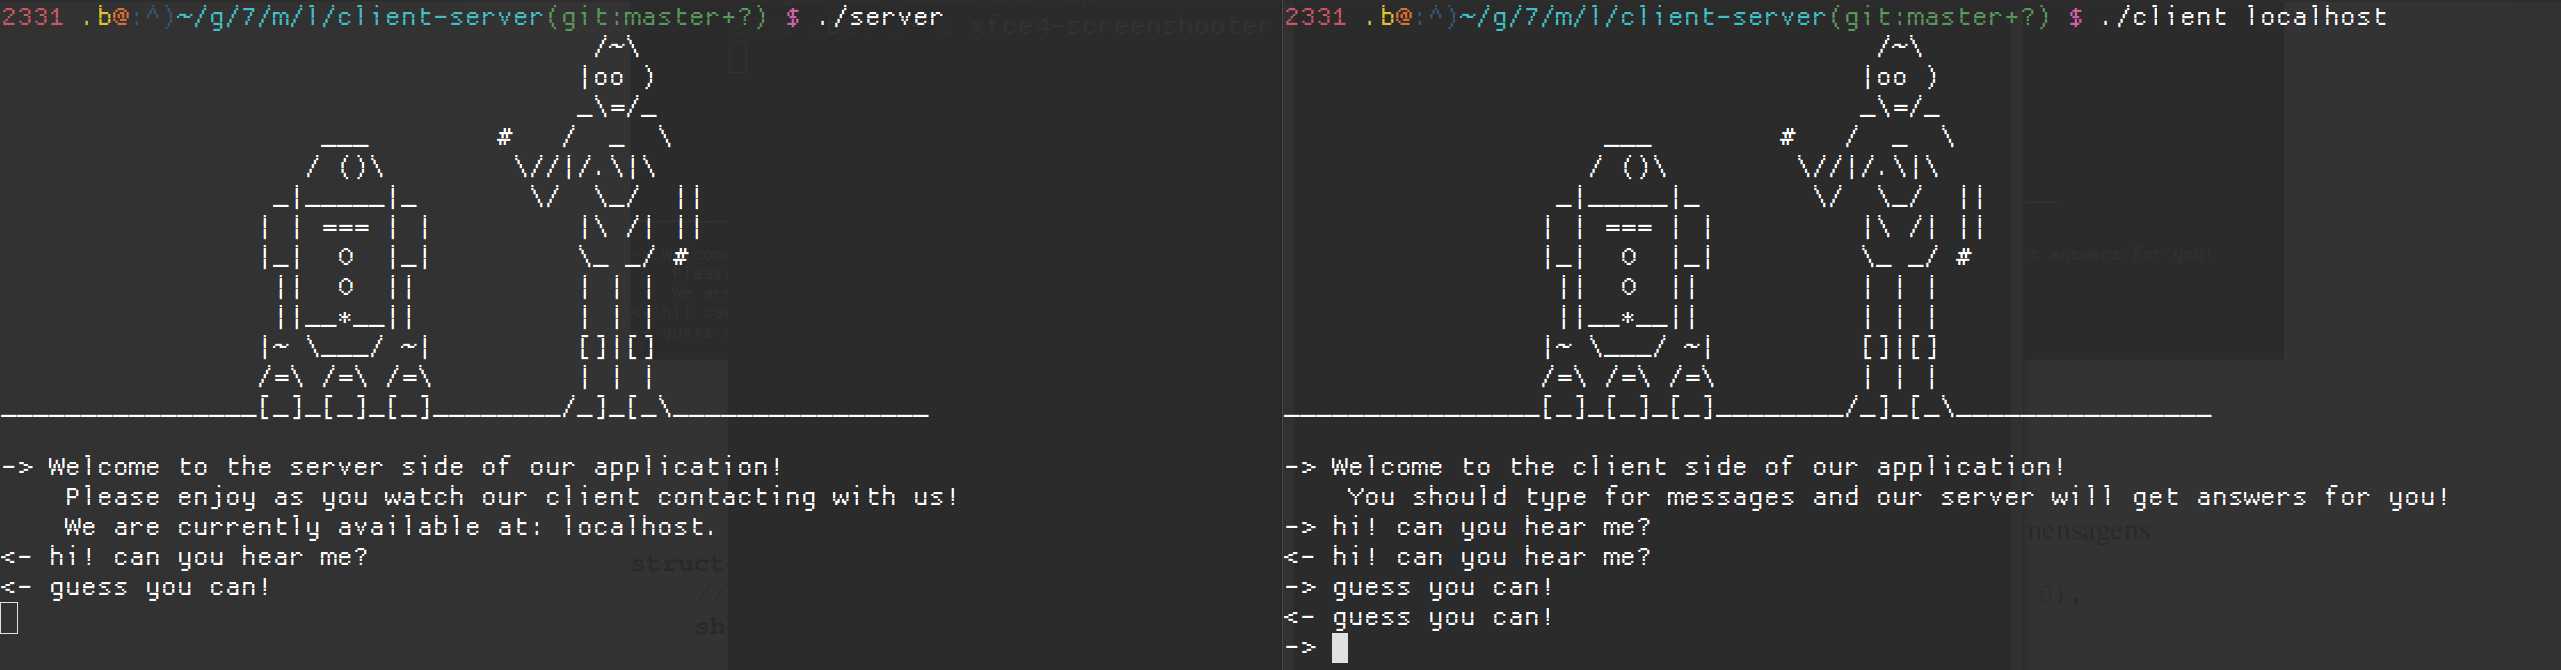
\includegraphics[width=1\textwidth]{img/sample.png}
    \caption{Exemplo de funcionamento do projeto}   
\end{center} 
\end{figure*}
%%%%%%%%%%%%%%%%%%%%%%%%%%%%%%%%%% page 2

%%% Introdução %%%%%%%%%%%%%%%%%%%%%%%%%%%%%%%%%%%%%%%%%%%%%%%%%%%%%%%%%%%%%%%%%%%
Neste projeto, foi implementado uma estrutura de comunicação entre cliente e servidor baseado em uma conexão TCP utilizando sockets na linguagem C. Nela, o cliente pode mandar mensagens de texto para o servidor que, ao confirmar o recebimento, retorna a mesma mensagem como um \textit{acknowledge} ao cliente.

%%% Seções %%%%%%%#####%%%%%%%%%%%%%%%%%%%%%%%%%%%%%%%%%%%%%%%%%%%%%%%%%%%%%%%%%%%
\section{client.c}
O cliente precisa executar os seguintes passos:

\begin{enumerate}
    \item Criar o socket de conexão;
    \item Estabelecer conexão com o servidor;
    \item Receber mensagem do usuário, mandar ao servidor e esperar resposta;
    \item Se algum erro ocorrer ou o cliente fechar a aplicação, fechar a conexão.
\end{enumerate}

 Para isso, utilizou-se funções da library \texttt{<netdb.h>}, que nos fornece 
 as implementações necessárias para criarmos a conexão com o servidor. 

 Para garantir o funcionamento da aplicação do cliente, foi estabelecida uma 
 interface em que o usuário digita uma mensagem, e recebe o \textit{acknowledge} 
 do cliente como retorno. Ambas as mensagens são exibidas na tela. Além disso, 
 caso qualquer erro tenha ocorrido no estabelecimento da conexão, um erro é 
 exibido e o programa é imediatamente interrompido.

 A seguir, serão detalhadas as funções utilizadas e seu contexto na 
 implementação do projeto.

\subsection{Criar o socket de conexão}

	\begin{lstlisting}[caption={Função utilizada para criação do socket}, label=Algorithm]
int socket(int domain, int type, int protocol);
	\end{lstlisting}

	\begin{lstlisting}[caption={Aplicação da função na implementação do projeto}, label=Algorithm]
/* create active socket */
s = socket(AF_INET, SOCK_STREAM, 0);
	\end{lstlisting}

	A função acima recebe como parâmetro a família da qual o endereço pertence (no nosso caso, IPv4), o tipo de socket (\texttt{SOCK\_STREAM}, que fornece streams de byte sequenciados, confiáveis e bidirecionais), e o protocolo a ser utilizado (0 significa que o socket vai utilizar um protocolo padrão apropriado para o tipo do socket requerido).

\subsection{Estabelecer conexão com o servidor}

	Para estabelecer a conexão com o servidor, primeiramente buscamos o host baseado no endereço fornecido pelo usuário:

	\begin{lstlisting}[caption={Função utilizada para acessar o endereço do host}, label=Algorithm]
/* get ip address */
host_address = gethostbyname(host);
if (host_address == NULL) {
    error("Invalid host name!\n");
}
	\end{lstlisting}

	Esta função nos retorna o endereço do servidor na forma de \texttt{struct\_hostent}, que pode retornar \texttt{NULL} em caso de não achar o servidor.

	A variável \texttt{host address} é do tipo \texttt{hostent} especificado abaixo:

	\begin{lstlisting}[caption={struct hostent}, label=Algorithm]
struct hostent {
	char* 	h_name;
	char** 	h_aliases;
	int 	h_addrtype;
	int 	h_length;
	char** 	h_addr_list;
	char* 	h_addr;
}
	\end{lstlisting}

	Contudo, apenas utilizamos \texttt{char *h\_ddr} para acessarmos o endereço do host ao realizar a conexão TCP.

	Assim, podemos utilizar a estrutura \texttt{sockaddr\_in} para especificarmos a porta e o endereço do host para a conexão:

	\begin{lstlisting}[caption={struct sockaddr\_in}, label=Algorithm]
struct sockaddr_in {
    // AF_INET, no nosso caso
    short            sin_family;

    // porta de conexao
    unsigned short   sin_port;

    // endereco do host
    struct in_addr   sin_addr;
    char             sin_zero[8];
};

	\end{lstlisting}

	\begin{lstlisting}[caption={Inicialização de endereço e porta}, label=Algorithm]
/* initialize data address */
bzero((char*) &socket_addr, 
        sizeof(socket_addr));
socket_addr.sin_family = AF_INET;
socket_addr.sin_port = htons(SERVER_PORT);
socket_addr.sin_addr = 
    *(struct in_addr*)host_address->h_addr;

	\end{lstlisting}


\subsection{Receber mensagem do usuário, mandar ao servidor e esperar resposta}
    Para estabelecer a comunicação com o usuário, foi utilizada, primeiramente,
a função \texttt{connect}, que permite a conexão do socket com a porta e o endereço
especificados em \texttt{socket\_addr}.

\begin{lstlisting}[caption={Estabelecimento da conexão com o servidor}, label=Algorithm]
valid(connect(s, (struct sockaddr*) &socket_addr, 
                        sizeof(socket_addr)), 
              "Failed...");
\end{lstlisting}

    Ao iniciar a conexão, é feita a transmissão de mensagens através do socket
para o servidor, com a função \texttt{send}, bastando especificar a mensagem a ser
comunicada. A captura da mensagem é feita pelo input do usuário, na própria tela.
    Em seguida, é chamada a função \texttt{recv}, que faz o papel de receber
o \textit{acknowledge} do servidor, com a resposta a ser imprimida na tela. Caso
nenhuma resposta tenha sido recebida, é assumido que a conexão foi finalizada e 
a aplicação é encerrada. Ao contrário, a troca de mensagens é realizada em loop.

\begin{lstlisting}[caption={Envio e recebimento de mensagens}, label=Algorithm]
/* send message */
valid(send(s, buff, strlen(buff), 0),
        "Failed...");

/* receive message */
int32_t len = recv(s, buff, MAX_LINE, 0);
valid(len, "Failed...");
\end{lstlisting}

\subsection{Se algum erro ocorrer ou o cliente fechar a aplicação, fechar a conexão}
    Para garantir que não ocorra nenhum erro conforme a aplicação está funcionando,
todas as chamadas de função para qualquer API de conexão com a internet possuem verificação
dos valores de retorno - e se eles fazem sentido com o contexto a qual a função foi chamada.

    Além disso, foi criada uma API simples para que os erros fossem exibidos na tela
de maneira uniforme e clara, automotizando o processo.

    \begin{lstlisting}[caption={API com verificação de erros, 
        utilizada tanto no cliente quanto servidor}, label=Algorithm]
void error(const char* msg) {
    fprintf(stderr, "\t[ERROR] %s", msg);
    exit(EXIT_FAILURE);
}

/* validate a status and report any errors */
void valid(int status, const char* msg) {
    if (status == ERROR) {
        error(msg);
    }
}
    \end{lstlisting}

    Caso o cliente deseje fechar a conexão, a conexão é finalizada através de nosso socket,
com a função \texttt{close}.

\section{server.c}
Semelhante ao comportamento do programa do cliente, o servidor foi divido em:

\begin{enumerate}
    \item Criar o socket passivo;
    \item Associação do socket com o descritor;
    \item Receber mensagem do cliente, exibi-las na tela e retorná-las
    \item Se algum erro ocorrer ou o cliente fechar a aplicação, fechar a conexão.
\end{enumerate}

    Foi estabelecida uma interface bem simples, que permite que o usuário veja as
    mensagens que serão ecoadas na tela - as quais correspondem às mensagens que
    o cliente envia através da conexão com o servidor.

\subsection{Criar o socket passivo}

Do mesmo modo que foi feito no cliente, foi criado um socket com a família da qual o endereço pertence (no nosso caso, IPv4), o tipo de socket (\texttt{SOCK\_STREAM}, que fornece streams de byte sequenciados, confiáveis e bidirecionais), e o protocolo a ser utilizado (0 significa que o socket vai utilizar um protocolo padrão apropriado para o tipo do socket requerido). O codigo usado é mostrado em \texttt{Code 2}.

\subsection{Associação do socket com o descritor}


\begin{lstlisting}[caption={Inicialização de endereço e porta}, label=Algorithm]
/* initialize data address */
bzero((char*) &socket_addr, sizeof(socket_addr));
socket_addr.sin_family = AF_INET;
socket_addr.sin_port = htons(CLIENT_PORT);
socket_addr.sin_addr.s_addr = htonl(INADDR_ANY);
	\end{lstlisting}

Para associar o socket com o descritor, foi utilizado a mesma estrutura do lado do cliente, mas modificando \texttt{sin\_port} e \texttt{s\_addr} para se conectar a qualquer endereço de cliente que faça o request para conexão. Assim, foi feito o bind do socket e o setou de modo que ele ouça por conexões:

\begin{lstlisting}[caption={Binding e Listening do socket}, label=Algorithm]
/* assign socket to a descriptor */
valid(bind(s, (struct sockaddr*) &socket_addr, 
         sizeof(socket_addr)),
        "Failed ...");

/* allow socket to accept connections */
valid(listen(s, MAX_PENDING),
        "Failed...");
\end{lstlisting}

\subsection{Receber mensagem do cliente, exibi-las na tela e retorná-las}


\begin{lstlisting}[caption={Estabelecimento de conexão e recebimento de mensagens}, label=Algorithm]
/* wait for connections and do my job! */
for ever {
    int32_t conn = 
    accept(s, (struct sockaddr*) NULL, NULL);

    valid(conn, 
    "Failed...");

    for ever {
        int32_t len = recv(conn, buff, MAX_LINE, 0);
        valid(len, 
            "Failed...");

        /* check if connection was terminated */
        if (len == 0) {
            fprintf(stdout, "Connection closed!\n");
            break; /* wait for another client */
        }

        /* set end on buff based on size */
        buff[len] = '\0';

        /* print text on screen */
        fprintf(stdout, "<- %s", buff);

        /* send back to client */
        if (send(conn, buff, len, 0) == ERROR) {
            printf("Failed to send echo to client!\n");
            break;
        }
    }

    close(conn);
}
	\end{lstlisting}

	Acima, temos a estrutura de código que espera por uma conexão, tenta estabelece-la e então espera por mensagens do cliente. \\

	Para estabelecer a conexão, ouvimos por algum request do seguinte modo:

	\begin{lstlisting}[caption={Estabelecimento de conexão}, label=Algorithm]
int32_t conn = accept(s, (struct sockaddr*) NULL, NULL);
valid(conn, "Failed to establish a connection from socket.\n");
	\end{lstlisting}

	Assim, ouvimos por uma conexão e, se não for possível se conectar, lançamos uma mensagem de erro. \\

	Se a conexão é estabelecida, esperamos por alguma mensagem do cliente, mostramos ela no servidor e mandamos ela devolta ao cliente:

	\begin{lstlisting}[caption={Estabelecimento de conexão}, label=Algorithm]
int32_t len = recv(conn, buff, MAX_LINE, 0);
valid(len, 
    "Failed to receive any message from my connection!\n");

/* check if connection was terminated */
if (len == 0) {
    fprintf(stdout, "Connection closed!\n");
    break; /* wait for another client */
}

/* set end on buff based on size */
buff[len] = '\0';

/* print text on screen */
fprintf(stdout, "<- %s", buff);

/* send back to client */
if (send(conn, buff, len, 0) == ERROR) {
    printf("Failed to send echo to client!\n");
    break;
}
	\end{lstlisting}

	Utilizamos a função \texttt{recv} para o recebimento da mensagem, checamos se a mensagem foi recebida corretamente, printamos no terminal do servidor e então utilizamos a função \texttt{send} para mandar a mesma mensagem devolta ao cliente.\\

\subsection{Se algum erro ocorrer ou o cliente fechar a aplicação, fechar a conexão}

Semelhante ao lado do servidor, utilizamos um conjunto de funções que lançam mensagens de erro caso algum ocorra, e utilizamos a função \texttt{close} para quando o erro demanda um fechamento da conexão

\section{Testes}

Para testarmos o funcionamento da estrutura, abrimos o processo do servidor e então do cliente e mandamos mensagens entre um e outro, como mostrado na \texttt{figura 1}. Então, testamos se as condições de erro foram corretamente implementadas, mandando endereços de servidores inexistentes ao cliente e fechando a aplicação do cliente para verificar se o servidor percebe o fechamento da conexão.

%%% References %%%%%%%%%%%%%%%%%%%%%%%%%%%%%%%%%%%%%%%%%%%%%%%%%%%%%%%%%%%%%%%%%
%%
{\small
\bibliographystyle{unsrt}
\bibliography{refs}
}

\end{document}